\subsection{平常時のグループ化の通信}
平常時のグループの通信フローを述べる.通信方式は,グループ内の通信にBLE,GLノードとGWノードの通信にLoRaWANを用いる.グループ内の通信は,インターバルが設けられ同期的に通信を行う.下記にシーケンス図\ref{fig:default_data_flow}を示す.

\begin{enumerate}
    \item GMノードはGLノードとの接続要求のため,Advを開始する.
    \item GLノードはGMノードとの接続確立のため,BLEにてScanを開始する.
    \item GLノードは接続確立後,GMノードからセンサデータを集約しGWへ送信する.
    \item WSNに新たなノードが参加した際にグループに所属するため,GLは自身のサービスUUIDを載せAdvを開始する.
\end{enumerate}

\begin{figure}[]
    \begin{center}
    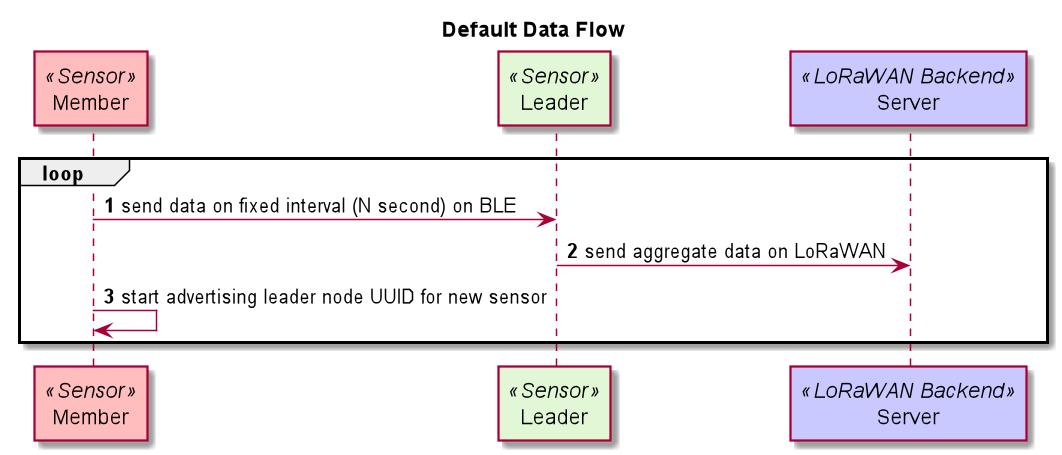
\includegraphics[width=13cm]{figures/グループ化の通信方式.png}
    \caption{グループ化の通信方式}
    \label{fig:default_data_flow}
    \end{center}
\end{figure}